\documentclass{article}

\usepackage{graphicx}
\usepackage{tikz}
\usepackage{tikzsymbols}
\usetikzlibrary{calc,patterns,shapes.geometric}
\pagestyle{empty}
\usepackage[margin=0pt]{geometry}
\geometry{papersize={14in,12in}}

\def\centerarc[#1](#2)(#3:#4:#5){\draw[#1] ($(#2)+({#5*cos(#3)},{#5*sin(#3)})$) arc (#3:#4:#5);}

\begin{document}
	\begin{figure}
		\centering
		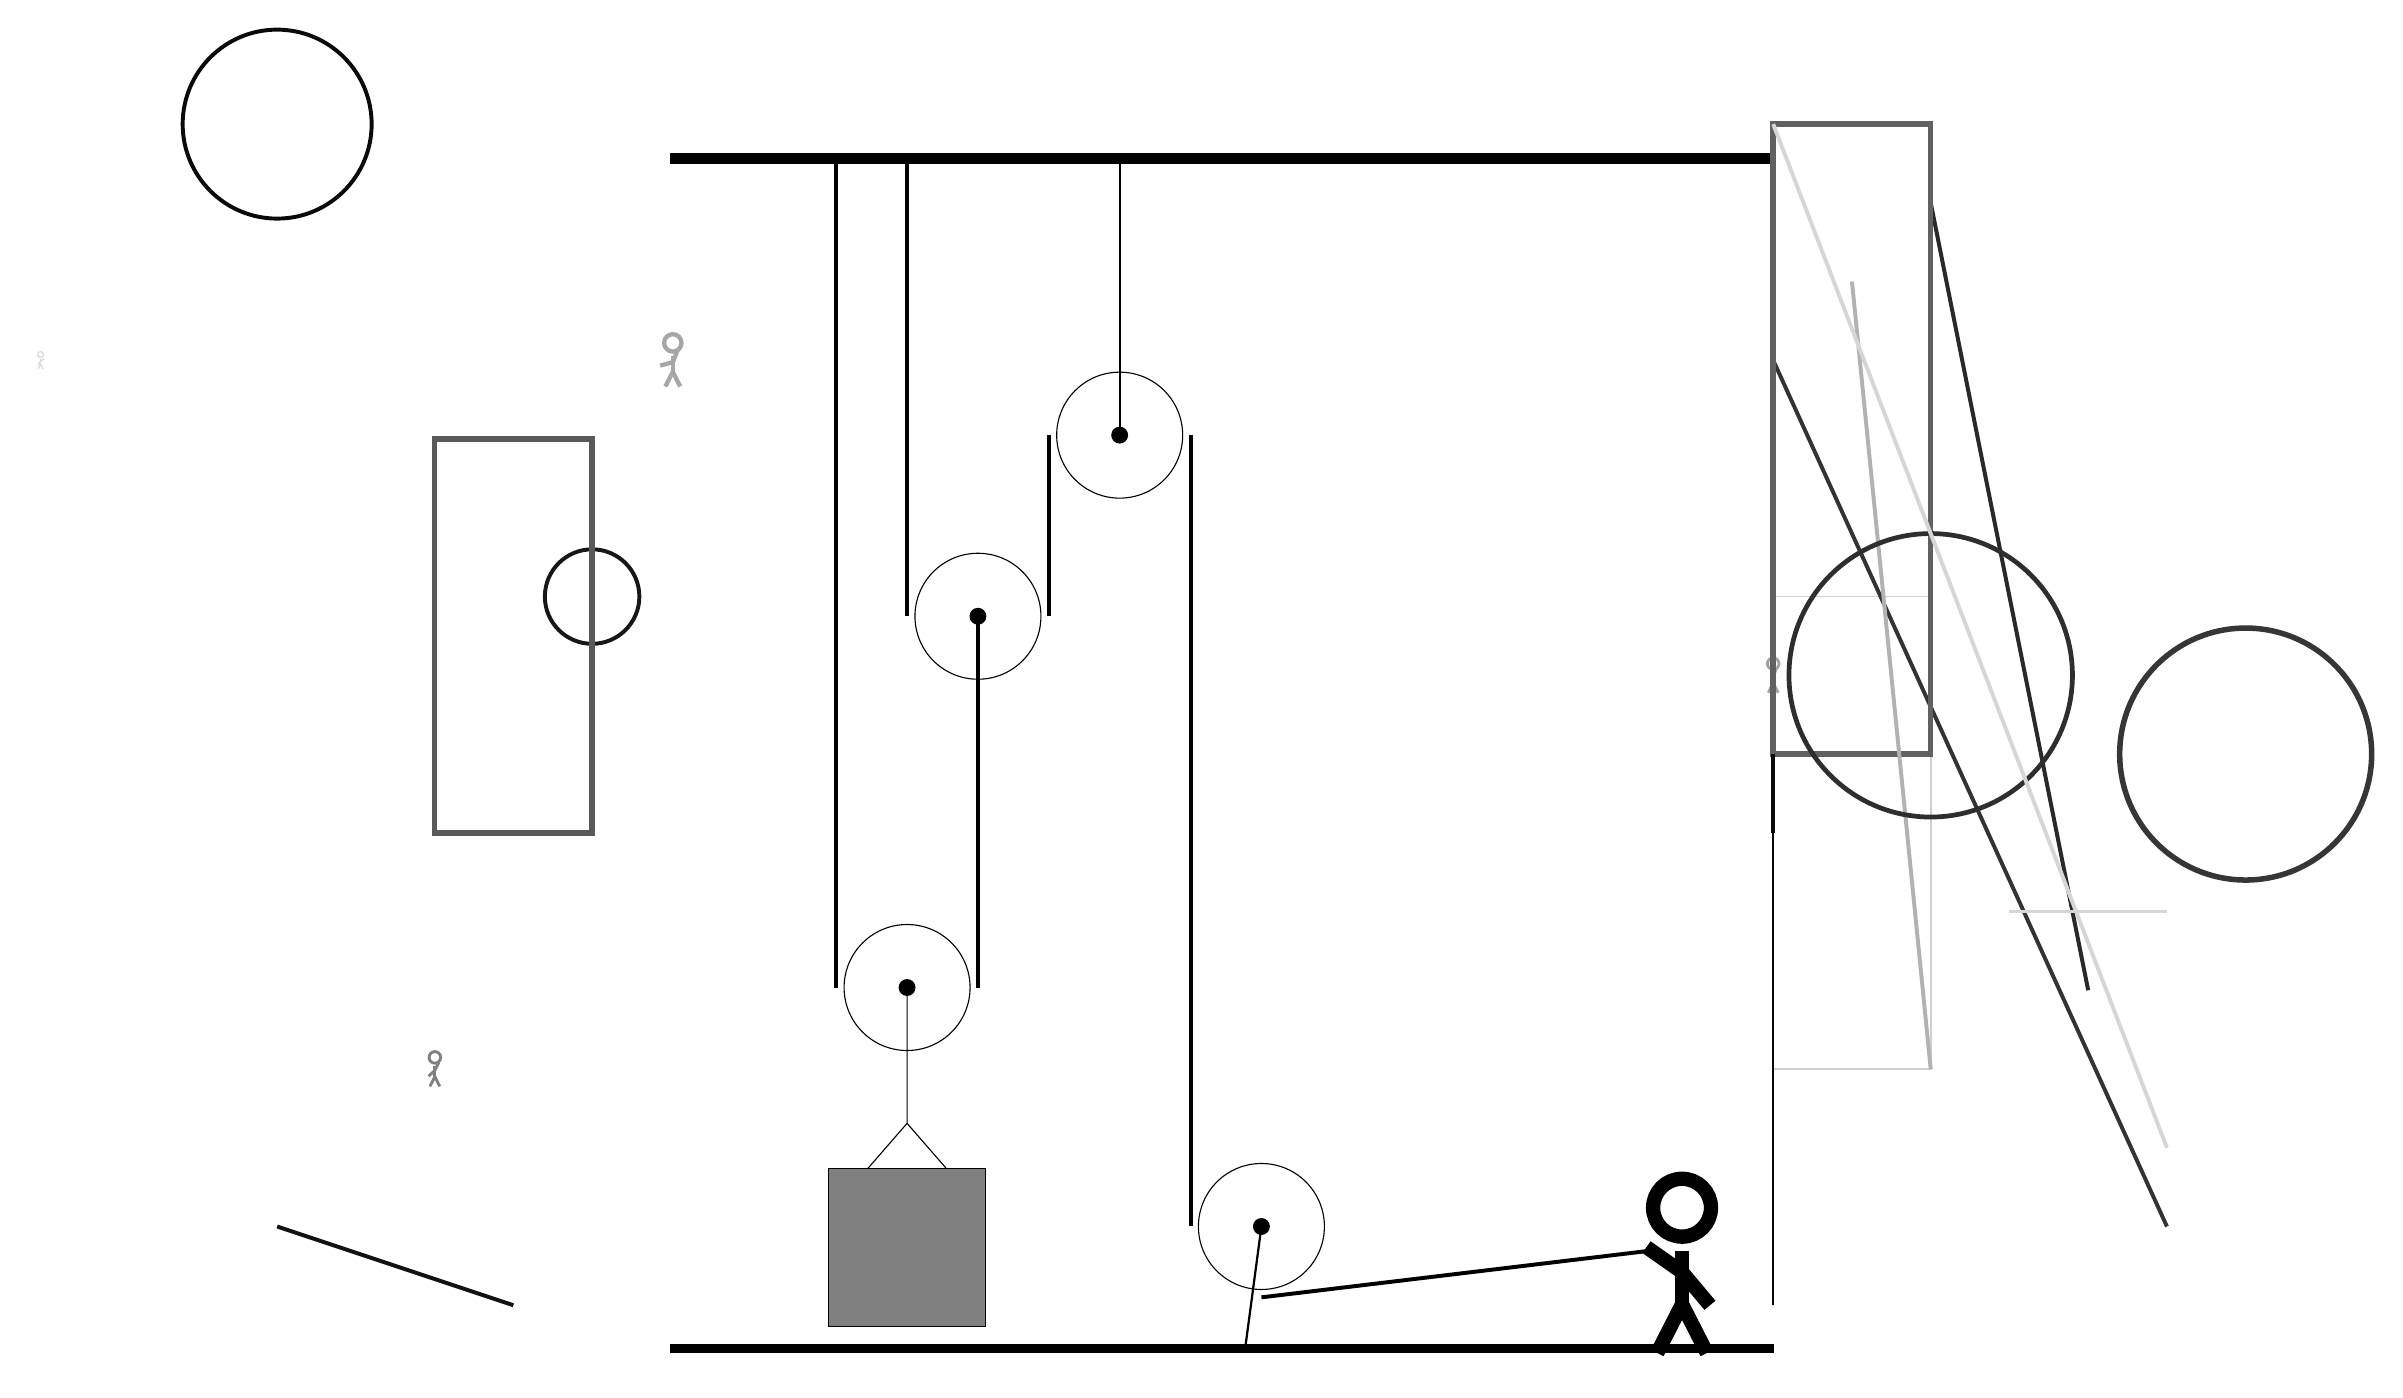
\begin{tikzpicture}
			%%%%% START %%%%%
			
			\draw[fill=black] (-2, 11.5) rectangle (12, 11.625);
			
			\draw (1, 1.035) circle (0.8);
			\draw[fill=black] (1, 1.035) circle (0.1);
			
			\draw (1.9, 5.75) circle (0.8);
			\draw[fill=black] (1.9, 5.75) circle (0.1);
			
			\node[line width=0.6mm, color=black!35] at (-2, 9) {\Strichmaxerl[3][15][68]};
			
			\draw [line width=0.5mm, color=black!91](-3, 6) circle (0.6);
			\draw[line width=0.5mm, color=black!93](-7, -2) -- (-4, -3);
			\draw[line width=0.2mm, color=black!19] (14, 0) rectangle (12, 6);
			
			\node[line width=0.7mm, color=black!36] at (12, 5) {\Strichmaxerl[2][83][68]};
			\draw[line width=0.5mm, color=black!84](14, 11) -- (16, 1);
			
			\draw[line width=0.5mm, color=black!80](17, -2) -- (12, 9);
			\draw[line width=0.7mm, color=black!62] (12, 12) rectangle (14, 4);
			\node[line width=0.5mm, color=black!14] at (-10, 9) {\Strichmaxerl[1][61][30]};
			
			\draw[line width=0.5mm, color=black!30](13, 10) -- (14, 0);
			\draw[line width=0.5mm, color=black!16](15, 2) -- (17, 2);
			
			\node[line width=0.6mm, color=black!50] at (-5, 0) {\Strichmaxerl[2][44][63]};
			\draw [line width=0.6mm, color=black!82](14, 5) circle (1.8);
			\draw [line width=0.5mm, color=black!96](-7, 12) circle (1.2);
			\draw[line width=0.5mm, color=black!16](12, 12) -- (17, -1);
			\draw[line width=0.5mm, color=black!96] (12, 4) rectangle (12, 3);
			
			\draw[line width=0.5mm, color=black!48](-7, 5) -- (-7, 5);
			\draw[line width=0.3mm, color=black!97] (12, 4) rectangle (12, -3);
			\draw[line width=0.7mm, color=black!65] (-3, 3) rectangle (-5, 8);
			
			\draw [line width=0.7mm, color=black!79](18, 4) circle (1.6);
			
			\draw (3.7, 8.05) circle (0.8);
			\draw[fill=black] (3.7, 8.05) circle (0.1);
			\draw[thick] (3.7, 8.05) -- (3.7, 11.5);
			
			\draw (5.5, -2) circle (0.8);
			\draw[fill=black] (5.5, -2) circle (0.1);
			\draw[thick] (5.5, -2) -- (5.3, -3.5);
			
			\draw (1, 1.035) -- (1, -0.69) -- (0.5, -1.265) -- (1.5, -1.265) -- (1, -0.69);
			\draw[fill=black!50] (0, -1.265) rectangle (2, -3.265);
			\draw[line width=0.5mm] (0.1, 11.5) -- (0.1, 1.035);
			\centerarc[line width=0.5mm](1, 1.035)(180:360:0.9);
			\draw[line width=0.5mm](1.9, 1.035) -- (1.9, 5.75);
			\draw[line width=0.5mm] (1.0, 11.5) -- (1.0, 5.75);
			\centerarc[line width=0.5mm](1.9, 5.75)(180:360:0.9);
			\draw[line width=0.5mm](2.8, 5.75) -- (2.8, 8.05);
			\centerarc[line width=0.5mm](3.7, 8.05)(0:180:0.9);
			\draw[line width=0.5mm] (4.6, 8.05) -- (4.6, -2);
			\centerarc[line width=0.5mm](5.5, -2)(0:90:-0.9);
			\draw[line width=0.5mm](5.5, -2.9) -- (10.5, -2.3);
			
			\node at (10.8, -2.5) {\Strichmaxerl[10][-35][-50]};
			
			\draw[fill=black] (-2, -3.5) rectangle (12, -3.6);
			
			%%%%% END %%%%%
		\end{tikzpicture}
	\end{figure}	
\end{document}